\documentclass[
%a4paper,12pt
encoding=utf8
]{./twoeskd}

% \usepackage{eskdappsheet}

% Packages required by doxygen
\usepackage[export]{adjustbox} % also loads graphicx
%\usepackage[utf8]{inputenc}
\usepackage{multicol}
\usepackage{multirow}
\usepackage{makeidx}
\usepackage{caption}
\usepackage{graphicx}



% NLS support packages
\usepackage[T2A]{fontenc}
\usepackage[russian]{babel}
\usepackage{pscyr}

% Font selection
\usepackage{courier}
\usepackage{amssymb}

% Page & text layout
% \usepackage{geometry}
% \geometry{%
%   a4paper,%
%   top=2.5cm,%
%   bottom=4.5cm,%
%   left=2.5cm,%
%   right=2.5cm%
% }
%\setlength{\emergencystretch}{15pt}
\setlength{\parindent}{0cm}
\setlength{\parskip}{0.2cm}

% Headers & footers
% \usepackage{fancyhdr}
% \pagestyle{fancyplain}
% \fancyhead[L]{\fancyplain{}{}}
% \fancyhead[C]{\fancyplain{}{\scriptsize\textbf{RU.17701729.509000 ТЗ 01-1-ЛУ}}}
% \fancyhead[R]{\fancyplain{}{}}
% \fancyfoot[L]{\fancyplain{}{}}
% \fancyfoot[C]{\fancyplain{}{}}
% \fancyfoot[R]{\fancyplain{}{}}

% debug to see the frame borders
% from https://en.wikibooks.org/wiki/LaTeX/Page_Layout
% \usepackage{showframe}

% Indices & bibliography
\usepackage{natbib}
\usepackage[titles]{tocloft}
\setcounter{tocdepth}{3}
\setcounter{secnumdepth}{5}


\newcommand\tab[1][1cm]{\hspace*{#1}}

% change style of titles in \section{}
\usepackage{titlesec}
\titleformat{\section}[hang]{\huge\bfseries\center}{\thetitle.}{1em}{}
\titleformat{\subsection}[hang]{\Large\normalfont\raggedright}{\thetitle.}{1em}{\underline}
\titleformat{\subsubsection}[hang]{\large\normalfont\raggedright}{\thetitle.}{1pt}{}

% Packages for text layout in normal mode
% \usepackage[parfill]{parskip} % автоматом делает пустые линии между параграфами, там где они есть в тексте
% \usepackage{indentfirst} % indent even in first paragraph
\usepackage{setspace}	 % controls space between lines
\setstretch{1} % space between lines
\setlength\parindent{0.9cm} % size of indent for every paragraph
\usepackage{csquotes}% превратить " " в красивые двойные кавычки
\MakeOuterQuote{"}


% this makes items spacing single-spaced in enumerations.
\newenvironment{my_enumerate}{
\begin{enumerate}
  \setlength{\itemsep}{1pt}
  \setlength{\parskip}{0pt}
  \setlength{\parsep}{0pt}}{\end{enumerate}
}


% Custom commands
% configure eskd
\titleTop{
\textbf{\Large ПРАВИТЕЛЬСТВО РОССИЙСКОЙ ФЕДЕРАЦИИ \\
НАЦИОНАЛЬНЫЙ ИССЛЕДОВАТЕЛЬСКИЙ УНИВЕРСИТЕТ \\
«ВЫСШАЯ ШКОЛА ЭКОНОМИКИ» } \\
\vspace*{0.2cm}
{\small Факультет компьютерных наук \\
Департамент программнoй инженерии \\
}
}
\titleDesignedBy{Студент группы БПИ 151 НИУ ВШЭ}{Куприянов  К.И.}
\titleAgreedBy{%
\parbox[t]{7cm} {
Доцент департамента \\
программной инженерии \\
факультета компьютерных наук \\
канд. техн. наук \\
}}{Ахметсафина Р. З.}
\titleApprovedBy{
\parbox[t]{10cm} {
Академический руководитель \\
образовательной программы \\
«Программная инженерия» \\
профессор департамента программной \\
инженерии канд. техн. наук \\
}}{Шилов В. В.}
\titleName{Игра — Эскейп Квест с Использованием Очков Виртуальной
    Реальности}
\workTypeId{RU.17701729.509000 51 01-1}

\titleSubname{Программа и методика испытаний}

% Custom packages
\usepackage{pdfpages}

\makeindex

%===== C O N T E N T S =====


\begin{document}
% Titlepage & ToC
\pagenumbering{roman}

% some water filling text, that is pointless but adds text
% 
\tab[0.75cm] Техническое задание – это основной документ, оговаривающий набор требований и
порядок создания программного продукта, в соответствии с которым производится разработка
программы, ее тестирование и приемка.

Настоящее Техническое задание на разработку ``Клиент-Серверное Android-Приложение для Управления Скидками в Розничных Сетях'' содержит следующие разделы: ``Введение'', ``Основания для разработки'',
``Назначение разработки'', ``Требования к программе'', ``Требования к программным документам'',
``Технико-экономические показатели'', ``Стадии и этапы разработки'', ``Порядок контроля и
приемки'' и приложения.

В разделе ``Введение'' указано наименование и краткая характеристика области применения
``Клиент-Серверного Android-Приложения для Управления Скидками в Розничных Сетях''.

В разделе ``Основания для разработки'' указан документ на основании, которого ведется
разработка и наименование темы разработки.

В разделе ``Назначение разработки'' указано функциональное и эксплуатационное
назначение программного продукта.

Раздел ``Требования к программе'' содержит основные требования к функциональным
характеристикам, к надежности, к условиям эксплуатации, к составу и параметрам технических
средств, к информационной и программной совместимости, к маркировке и упаковке, к
транспортировке и хранению, а также специальные требования.

Раздел ``Требования к программным документам'' содержит предварительный состав
программной документации и специальные требования к ней.

Раздел ``Технико-экономические показатели'' содержит ориентировочную экономическую
эффективность, предполагаемую годовую потребность, экономические преимущества разработки
``Клиент-Серверного Android-Приложения для Управления Скидками в Розничных Сетях''.

Раздел ``Стадии и этапы разработки'' содержит стадии разработки, этапы и содержание
работ.

В разделе ``Порядок контроля и приемки'' указаны общие требования к приемке работы.

Настоящий документ разработан в соответствии с требованиями:\\
1) ГОСТ 19.101-77 Виды программ и программных документов \cite{gost_types_of_software};\\
2) ГОСТ 19.102-77 Стадии разработки \cite{gost_stages_of_devel};\\
3) ГОСТ 19.103-77 Обозначения программ и программных документов \cite{gost_marking_software};\\
4) ГОСТ 19.104-78 Основные надписи \cite{gost_main_signs};\\
5) ГОСТ 19.105-78 Требования к программным документам \cite{gost_demands_for_docs};\\
6) ГОСТ 19.201-78 Техническое задание. Требования к содержанию и оформлению \cite{gost_tz}.\\

Изменения к данному Техническому заданию оформляются согласно ГОСТ 19.603-78 \cite{gost_main_rules_change},
Перед прочтением данного документа рекомендуется ознакомиться с терминологией,
приведенной в Приложении 1 настоящего технического задания.


\newpage
\pagenumbering{arabic}
\tableofcontents
% \pagenumbering{arabic}

% --- add my custom headers ---
\newpage
\section{Объект испытаний}
\subsection{Наименование программы}
Наименование программы на русском:
``Клиент-Серверное Android-Приложение для Управления Скидками в Розничных
Сетях''. \\
Наименование на английском:
``The Client-Server Android Application for Managing the Products' Discounts in
Retail Networks''.


\subsection{Краткая характеристика}
Программа предназначена для пользователей смартфонов на базе платформы Android.
Цель работы - создать удобное приложения для составления списков покупок,
добавления в них любых товаров (даже тех, которых нет в магазине), отслеживания
акций, а так же просмотра всех акций в нескольких магазинах. Это позволит
пользователям экономить свои средства на ежедневных покупках и быть в курсе
актуальных акций магазинов.  Серверная часть приложения должна представлять из
себя web-crawler для сбора данных с сайтов розничных сетей. Crawler должен
иметь модульную структуру, для быстрого восстановления после изменения дизайна
сайтов. Должен быть реализован механизм взаимодействия с клиентами посредством
обменивания файлами в формате JSON.\\
Главной чертой данного приложения
является его лёгкая, быстрая масштабируемость и модульность программного кода.



\newpage
\section{Цель испытаний}
Цель проведения испытаний заключается в проверке выполнения заявленных в
техническом задании требований к программной документации и составу выполняемых
функций программы, надежности и корректности ее работы, а также интерфейсу и
внешнему виду приложения.

\newpage
\section{Требования к програмному изделию}
Требования к программе представлены в документах:
\begin{my_enumerate}
    \item Клиент-Серверное Android-Приложение для Управления Скидками в Розничных Сетях. Техническое Задание.
    \item Клиент-Серверное Web-Приложение для Управления Скидками в Розничных Сетях. Техническое Задание.
\end{my_enumerate}

% EOF



\newpage
\section{Требования к програмной документации}
\subsection{Предварительный состав программной документации}
\begin{my_enumerate}
    \item «Игра - Эскейп Квест с Использованием Очков Виртуальной Реальности». Техническое задание
    \item «Игра - Эскейп Квест с Использованием Очков Виртуальной Реальности». Пояснительная записка
    \item «Игра - Эскейп Квест с Использованием Очков Виртуальной Реальности». Руководство оператора
    \item «Игра - Эскейп Квест с Использованием Очков Виртуальной Реальности». Программа и методика испытаний
    \item «Игра - Эскейп Квест с Использованием Очков Виртуальной Реальности».  Текст программы
\end{my_enumerate}



\newpage
\section{Средства и порядок испытаний}
%=========================================
\subsection{Параметры технических средств, используемых во время испытаний}
Для испытания программы необходимо учесть следующие системные требования:
\begin{my_enumerate}
    \item Мобильный телефон со следующими минимальными требованиями:
    \begin{my_enumerate}
        \item Операционная система Android версии 4.4.4 KitKat и выше (API level 19+)
        \item 64-разрядный (x64) процессор
        \item 1ГБ оперативной памяти (ОЗУ)
        \item 100 МБ свободного места на внутреннем накопителе
        \item Наличие гироскопа
        \item Наличие акселерометра
        \item Размеры устройства не более 165мм х 90 мм
        \item Длина устройства не менее 135мм
    \end{my_enumerate}
    \item Любая модель Cardboard (Google Cardboard)
\end{my_enumerate}


%=========================================
\subsection{Порядок проведения испытаний}
Испытания проводятся поэтапно, друг за другом, в следующем порядке:
\begin{my_enumerate}
    \item Испытание выполнения требований к программной документации
    \item Испытание выполнения требований к графическому интерфейсу и оформлению программы
    \item Испытание выполнения требований к функциональным характеристикам программы, надежности и корректности ее работы
    \item Испытание выполнения требований к временным характеристикам
\end{my_enumerate}


%=========================================
\subsection{Условия проведения испытаний}

\subsubsection{Требования к численности и калификации персонала}
Минимальное количество персонала, требуемого для работы программы: 1 оператор. Пользователь данного программного продукта должен разбираться в работе мобильных устройств, уметь устанавливать и удалять программы, запускать их. Перед использованием программы пользователь должен заранее проинструктирован и уведомлен о составе выполняемых функций и других характеристиках приложения.





\newpage
\section{Методы испытаний}
Испытания представляют собой процесс установления соответствия программы и
программной документации заданным требованиям.

\subsection{Проверка требований к документации}
Проверяется наличие всех документов перечисленных в пyнкте 4.1 данного
документа и их соответствие ГОСТ.

\subsection{Проверка требований к интерфейсу}
Интерфейс должен соответствовать схеме, указанной в настоящем Техническом
Задании и быть совместим а ОС Андроид. Использованные графические элементы
должны быть стандартными элементами графического семейства системы Андроид.
Используемая цветовая палитра должна соответствовать рекомендациям сайта,
указанного в настоящем Техническом Задании. Рис.~\ref{interface}

\begin{figure}[h!]
    \centering
    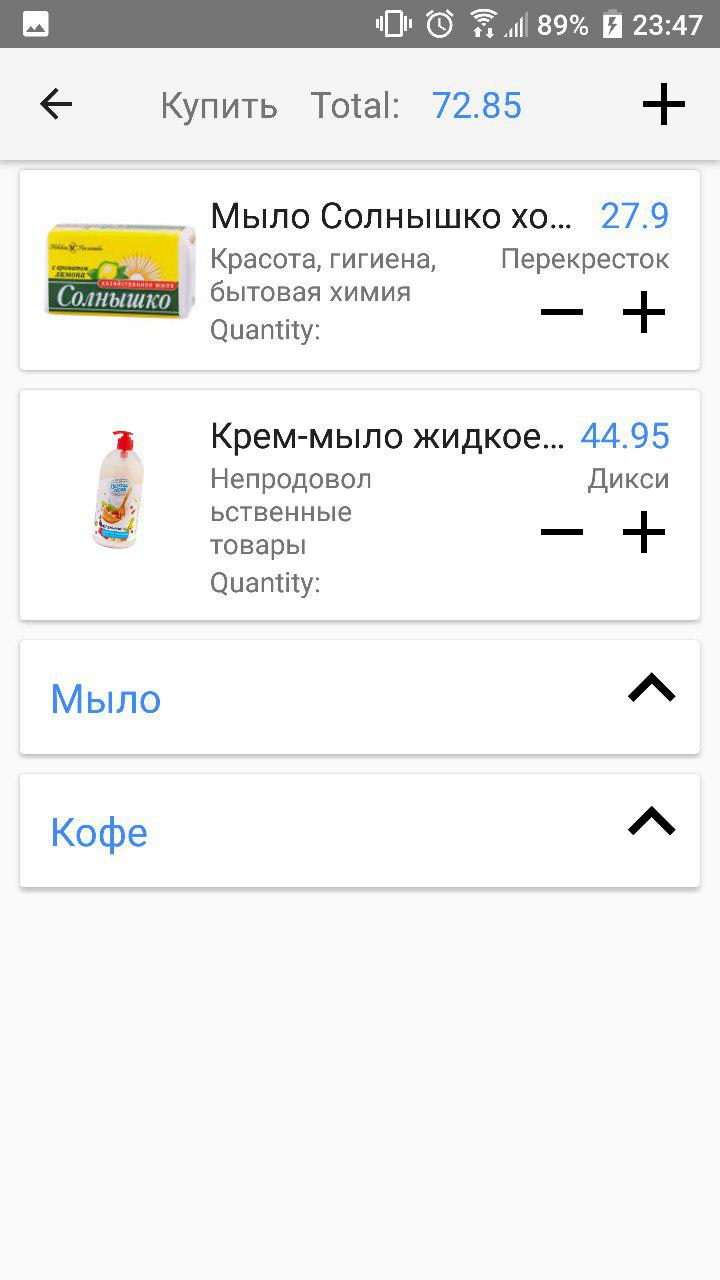
\includegraphics[height=0.48\textheight]{./screenshots/3/shoplist.jpg}
    \caption{проверка требований к интерфейсу}
    \label{interface}
\end{figure}

\newpage
\subsection{Проверка требований к функциональным характеристикам}

\subsubsection{Андроид приложение}
Проверка реализованного функционала продемонстрирована на скриншотах ниже.

Должна быть реализованa возможность просмотра списка доступных магазинов с
акционными товарами (выпадающий список на Рис.~\ref{items}), представление текущих акций для конкретного магазина в
виде общего списка и по категориям. (Рис.~\ref{categs_1},~\ref{categs_2}) Должна быть реализована постепенная
загрузкa товаров магазинов (по страницам) для экономии трафика и меньшей
нагрузкой на мобильное устройство.

Загрузка акций не должна превышать лимит, установленный требованиями и проверена в
пункте 6.4 настоящей Программы и Методики Испытаний.

\begin{figure}[h!]
    \centering
    \minipage{0.3\textwidth}
    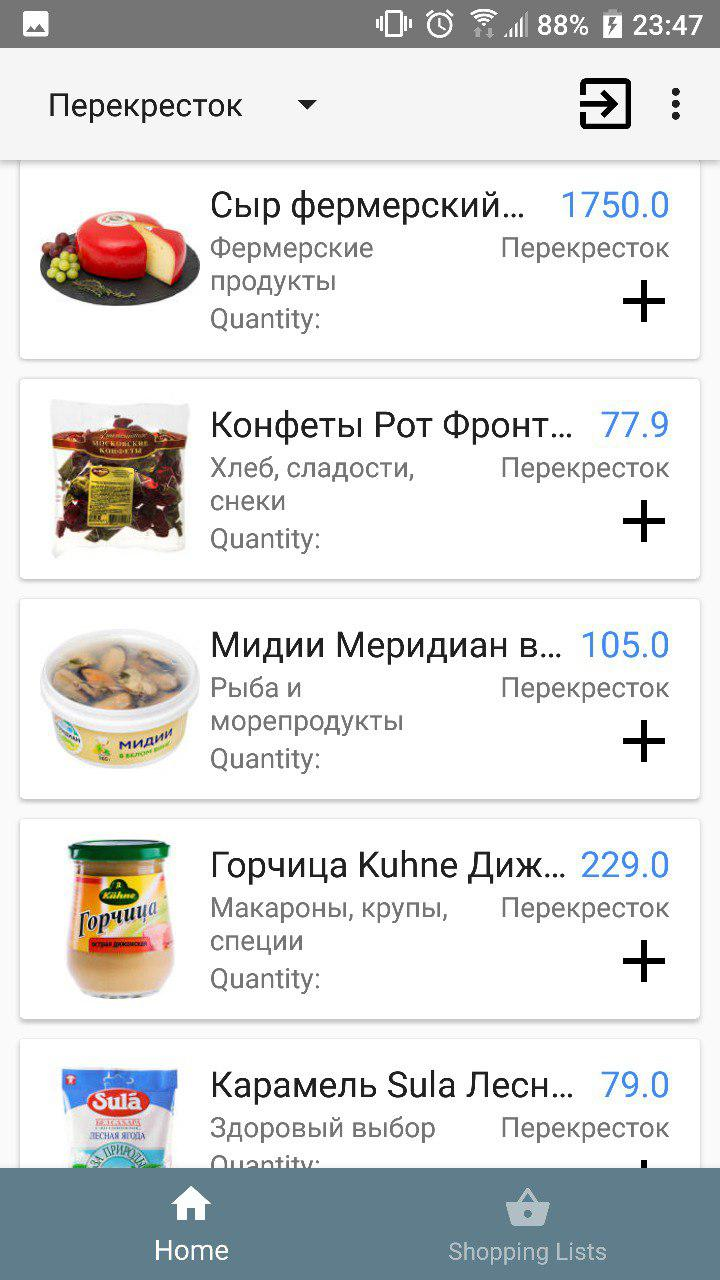
\includegraphics[height=0.38\textheight]{./screenshots/3/home.jpg}
    \caption{\small{просмотр всех акций}}
    \label{items}
    \endminipage\hfill
    \minipage{0.3\textwidth}
    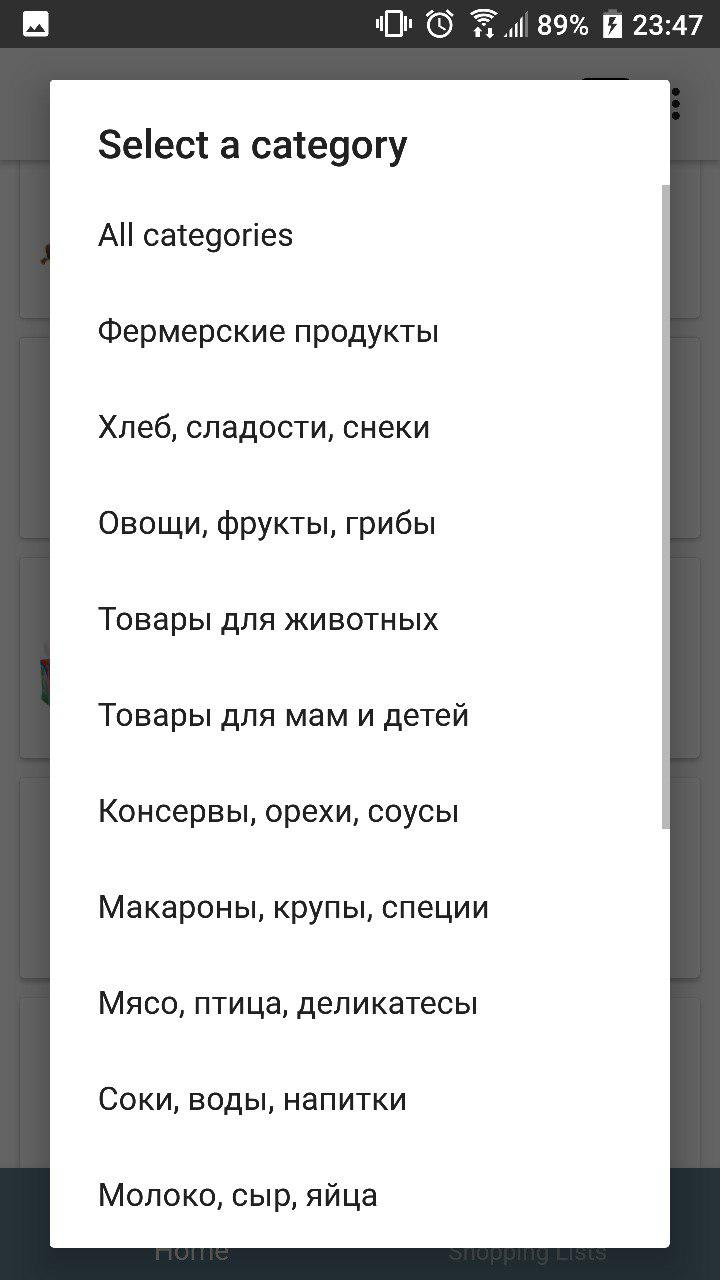
\includegraphics[height=0.38\textheight]{./screenshots/3/categories.jpg}
    \caption{\small{выбор категории}}
    \label{categs_1}
    \endminipage\hfill
    \minipage{0.3\textwidth}
    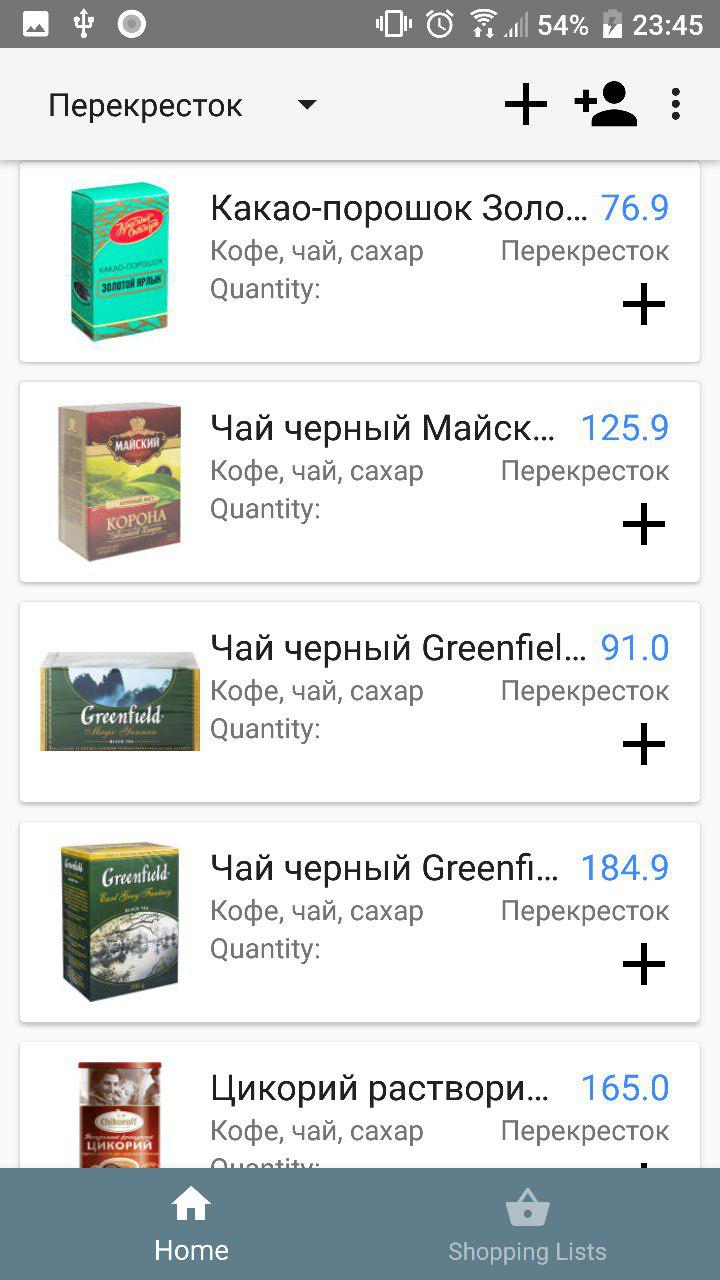
\includegraphics[height=0.38\textheight]{./screenshots/3/categ_filter.jpg}
    \caption{\small{просмотр по категориям. На скриншоте --- категория ``Кофе, чай, сахар''}}
    \label{categs_2}
    \endminipage{}
\end{figure}

Должна быть реализована возможность создания списков покупок c разными названиями,
и возможность удаления списка покупок. (Рис.~\ref{sl_all} -~\ref{delete_sl})

\begin{figure}[h!]
    \centering
    \minipage{0.3\textwidth}
    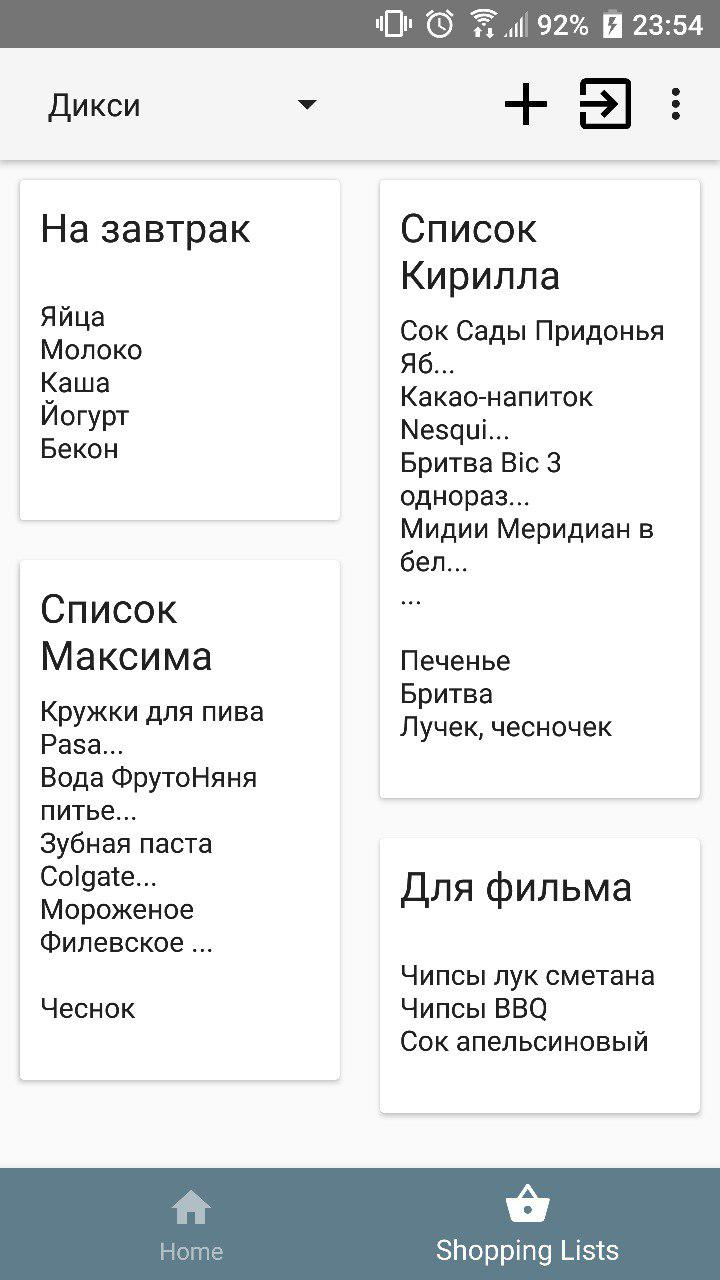
\includegraphics[height=0.38\textheight]{./screenshots/3/all_shoplists.jpg}
    \caption{\small{просмотр всех списков покупок}}
    \label{sl_all}
    \endminipage\hfill
    \minipage{0.3\textwidth}
    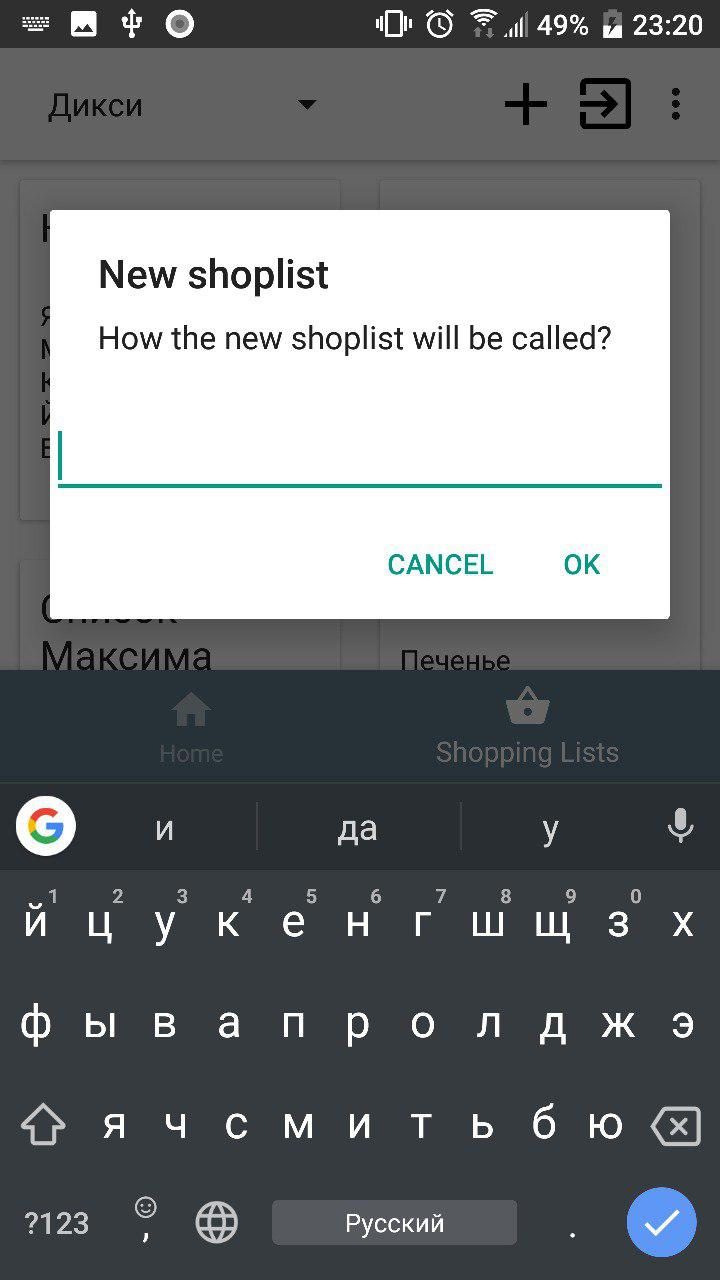
\includegraphics[height=0.38\textheight]{./screenshots/3/new_shoplist.jpg}
    \caption{\small{создание нового списка покупок}}
    \endminipage\hfill
    \minipage{0.3\textwidth}
    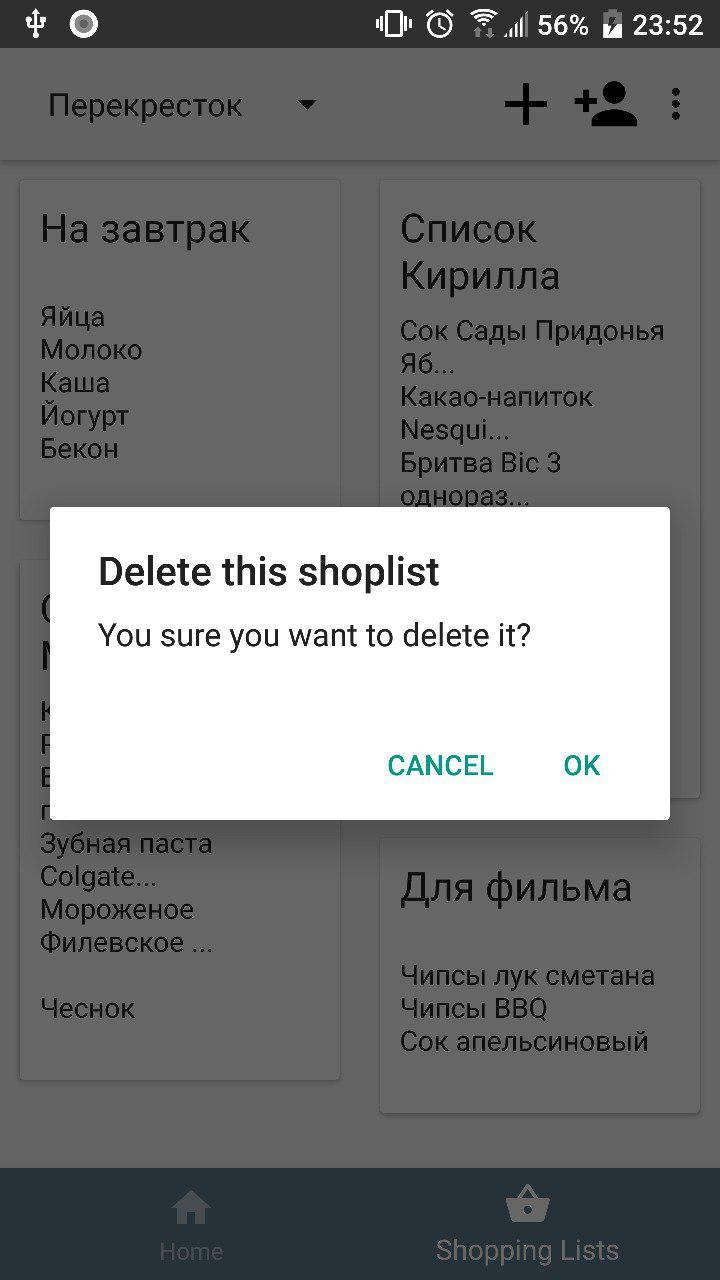
\includegraphics[height=0.38\textheight]{./screenshots/3/delete_shoplist.jpg}
    \caption{\small{удаление списка покупок}}
    \label{delete_sl}
    \endminipage{}
\end{figure}

Добавление товара в список покупок должна вызываться нажатием кнопки '+', а
удалениe товара из списка покупок путём нажатия кнопки '-'.

Добавление в список
покупок пользовательских товаров, которых нет в магазине вызывается нажатием
'+' из списка покупок, а просмотр подобранных программой товаров согласно
запросу пользователя должен вызываться нажатием на пользовательский товар.
Рис~\ref{custom}

При долгом зажатии подобранных товаров должно происходить добавление
подобранных товаров в список покупок.

При переходе на фрагмент 2 (Списки покупок), на экране устройства должно
показываться предварительное отображение элементов каждого списка покупок до их
открытия.

\begin{figure}[h!]
    \centering
    \minipage{0.3\textwidth}
    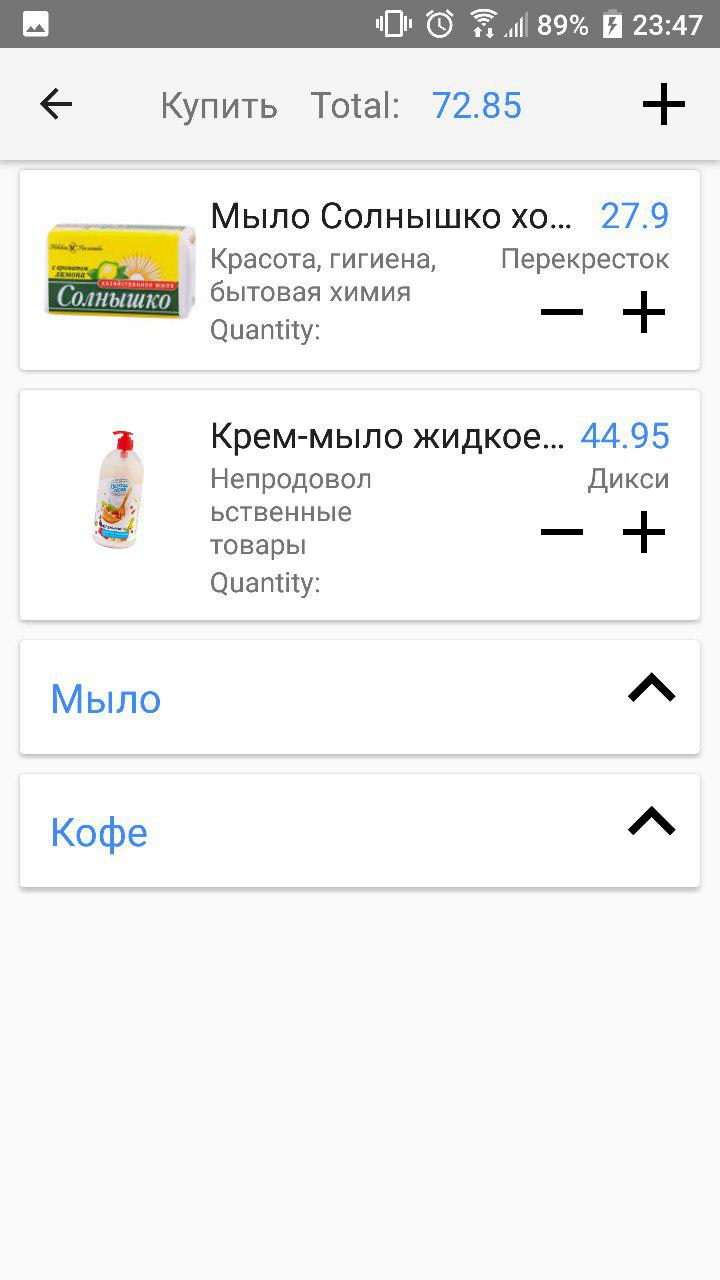
\includegraphics[height=0.38\textheight]{./screenshots/3/shoplist.jpg}
    \caption{\small{просмотр конкретного списка покупок}}
    \endminipage\hfill
    \minipage{0.3\textwidth}
    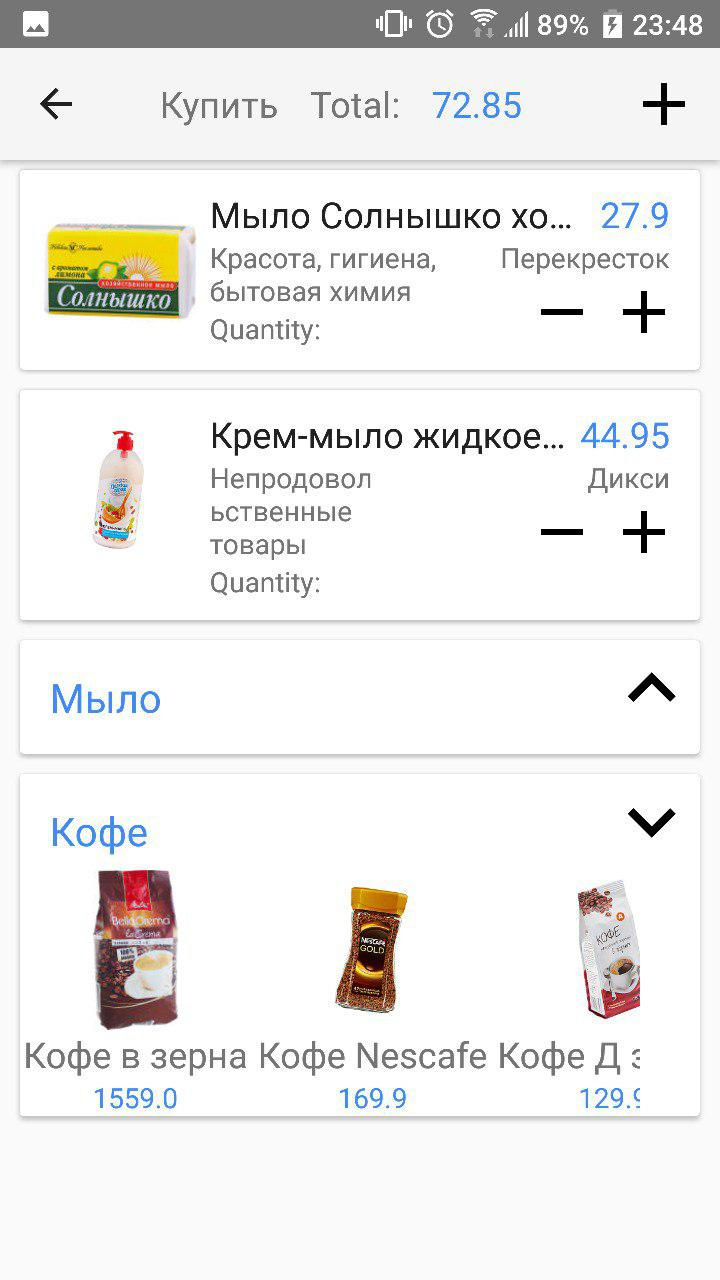
\includegraphics[height=0.38\textheight]{./screenshots/3/shoplist_custom_fold.jpg}
    \caption{\small{просмотр подобранных программой товаров в соответствии с запросом пользователя}}
    \label{custom}
    \endminipage\hfill
    \minipage{0.3\textwidth}
    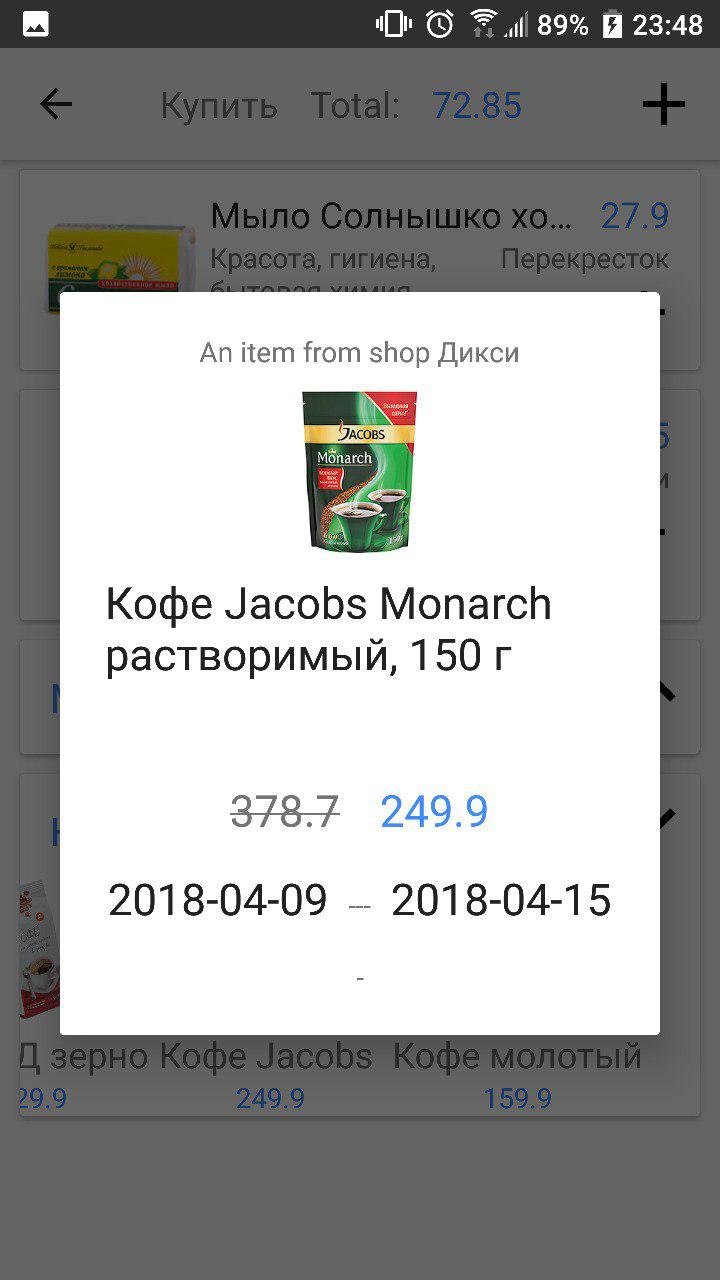
\includegraphics[height=0.38\textheight]{./screenshots/3/full_item_preview.jpg}
    \caption{\small{просмотр всей информации о товаре}}
    \endminipage{}
\end{figure}

На экране с активностью RegisterActivity (Рис.~\ref{register}) должна быть возможность регистрации
через мобильное приложение, а на экране LoginActivity (Рис.~\ref{register}) --- вход в аккаунт через
мобильное приложение, возможность смены аккаунта должна осуществляться путём 1) выхода из аккаунта 2) входа в другой аккаунт.

\begin{figure}[h!]
    \centering
    \minipage{0.45\textwidth}
    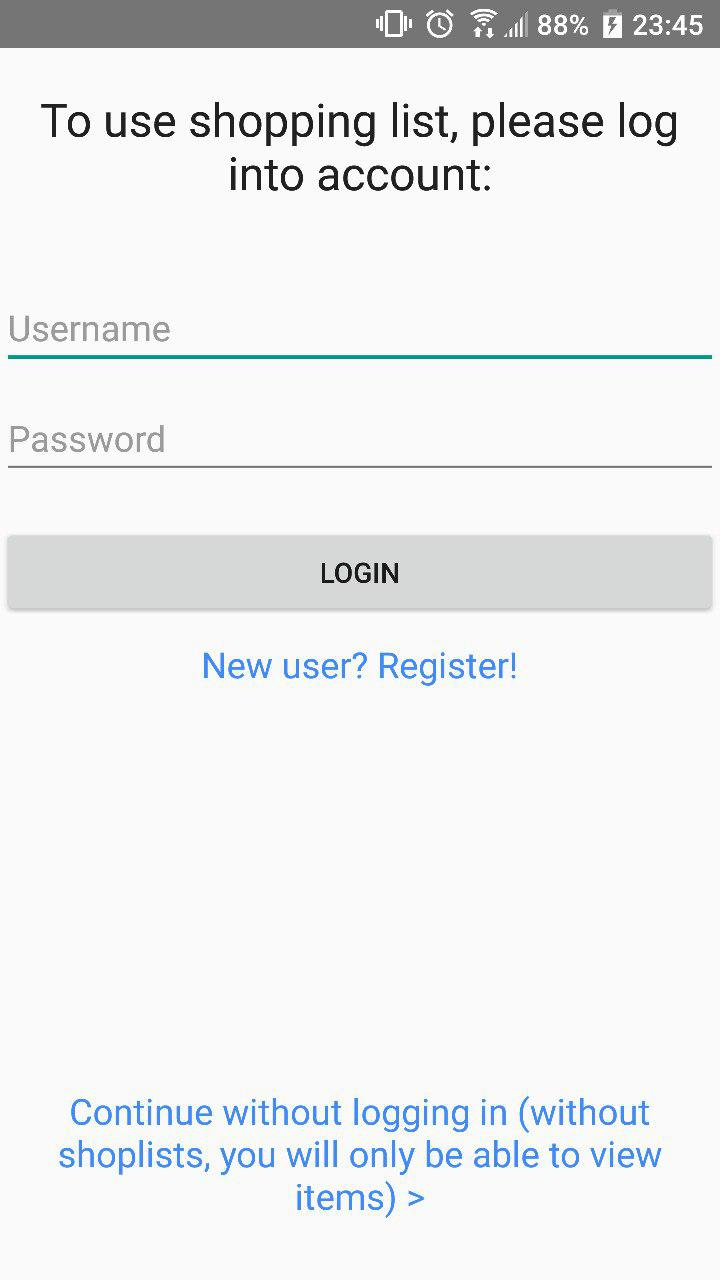
\includegraphics[height=0.42\textheight]{./screenshots/3/login.jpg}
    \caption{\small{вход в аккаунт}}
    \label{login}
    \endminipage\hfill
    \minipage{0.45\textwidth}
    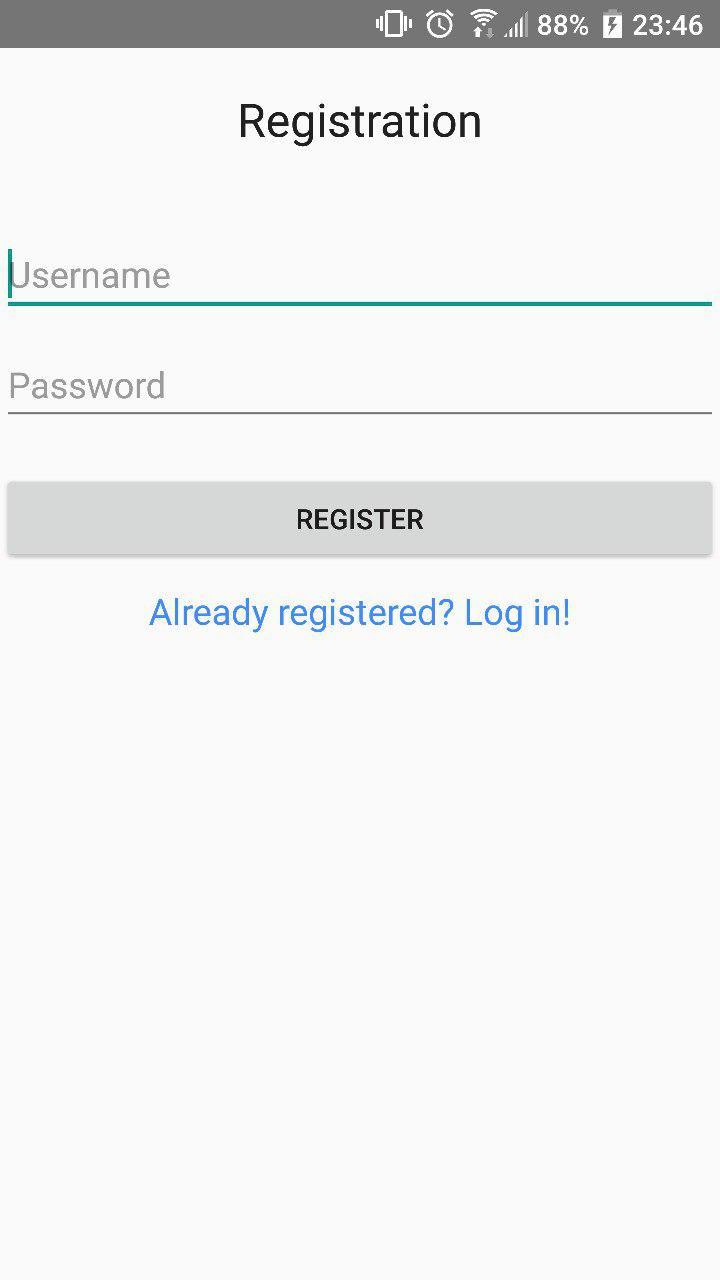
\includegraphics[height=0.42\textheight]{./screenshots/3/register.jpg}
    \caption{\small{регистрация аккаунта}}
    \label{register}
    \endminipage{}
\end{figure}


При долгом нажатии на элементы
управления button (кнопка) должны появляться всплывающие подсказки. (Рис.~\ref{hint})

Должен быть реализован обучающий фрагмент в разделе help (), содержащий руководство
пользователя по управлению программой. (Рис.~\ref{help})
Должно быть отображение индикатора процесса загрузки данных с сервера,
При отсутствии интернет-соединения должно происходить перенаправление в настройки сети для
последующего включения интернета .

\begin{figure}[h!]
    \centering
    \minipage{0.3\textwidth}
    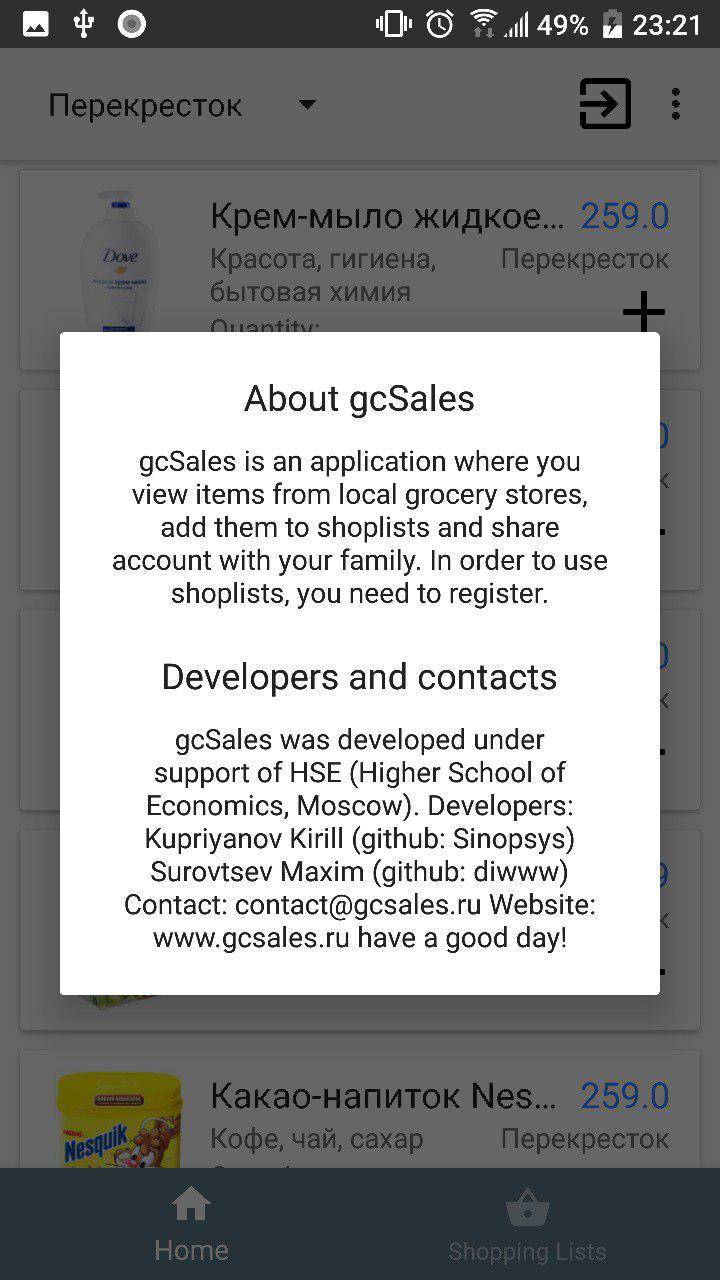
\includegraphics[height=0.38\textheight]{./screenshots/3/about.jpg}
    \caption{\small{просмотр раздела ``о приложении''}}
    \endminipage\hfill
    \minipage{0.3\textwidth}
    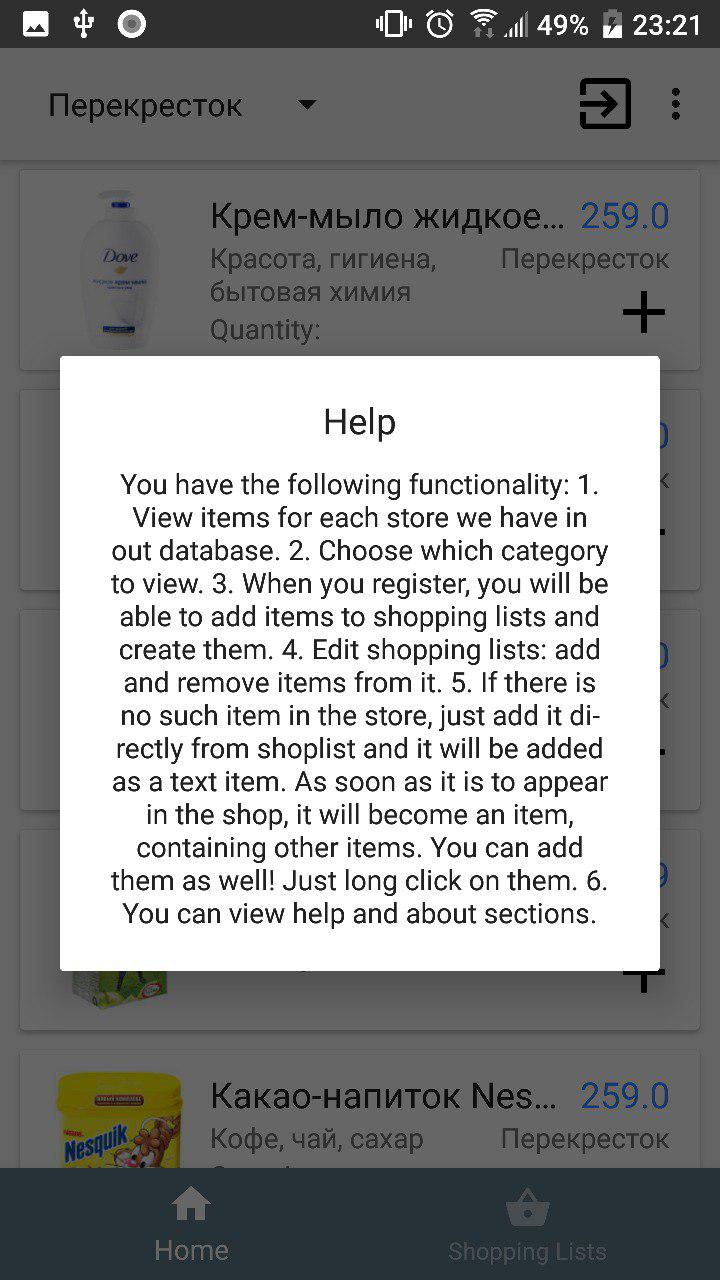
\includegraphics[height=0.38\textheight]{./screenshots/3/help.jpg}
    \caption{\small{просмотр подсказки пользования приложением}}
    \label{help}
    \endminipage\hfill
    \minipage{0.3\textwidth}
    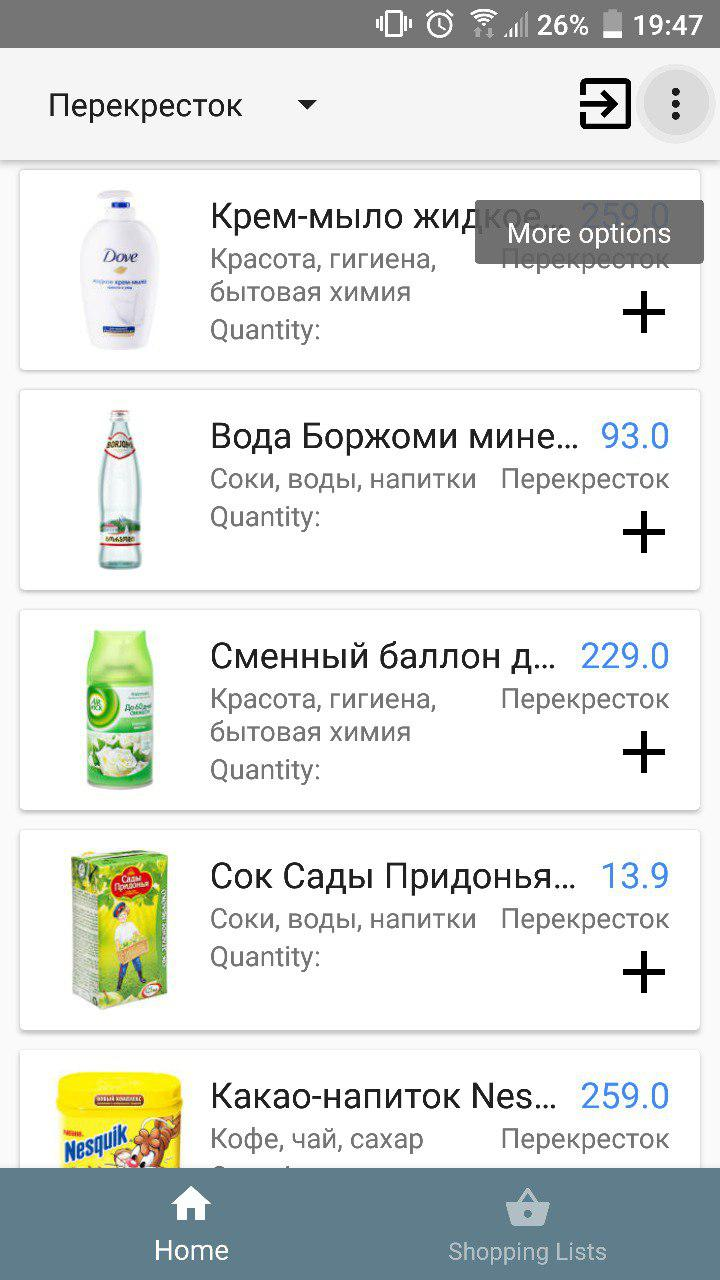
\includegraphics[height=0.38\textheight]{./screenshots/3/hint.jpg}
    \caption{\small{просмотр всплывающего описания элементов button (кнопок)}}
    \label{hint}
    \endminipage{}
\end{figure}

\newpage
\subsubsection{Crawler}
Все необходимые для реализации программы модули должны быть реализованы (Рис.~\ref{tree})

\begin{figure}[h!]
    \centering
    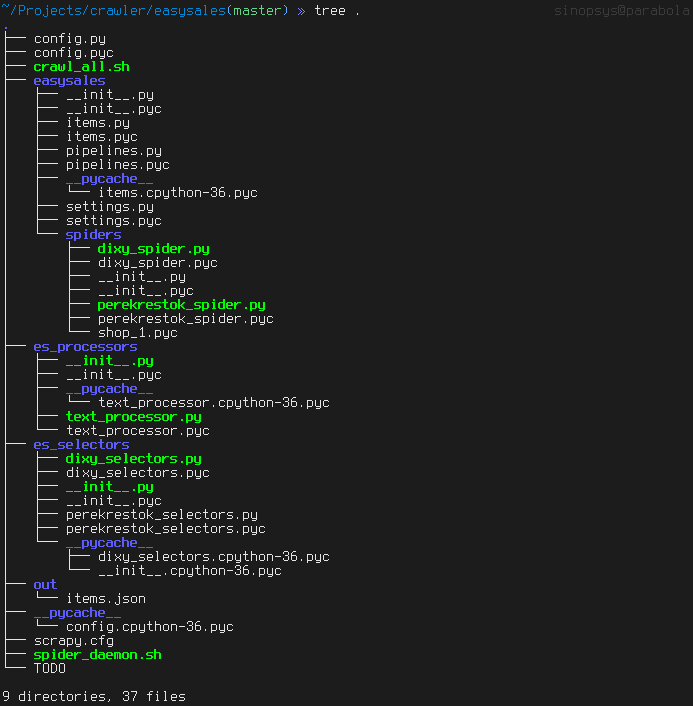
\includegraphics[width=0.56\textwidth]{./screenshots/3/tree.png}
    \caption{\small{структура проекта crawler'a}}
    \label{tree}
\end{figure}

\newpage
Работа crawler'a на Рис.~\ref{crawl_dixy}. При запуске всё работает должно
работать по описанному в настоящей Пояснительной Записке алгоритму, запросы
должны отправляться на сервер.

\begin{figure}[h!]
    \centering
    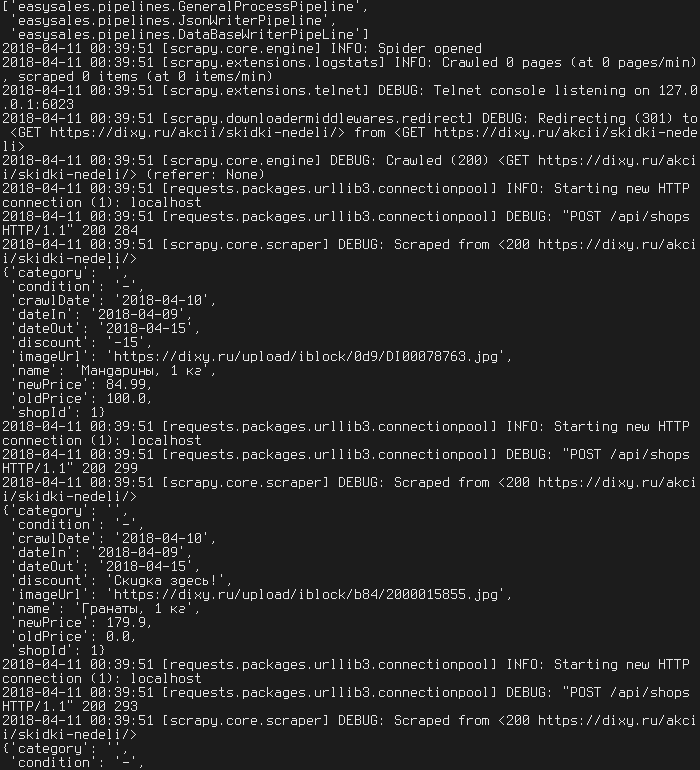
\includegraphics[width=0.9\textwidth]{./screenshots/3/crawl_dixy.png}
    \caption{\small{начало запуска crawler'a}}
    \label{crawl_dixy}
\end{figure}


\newpage
\subsection{Проверка требований к временным характеристикам}
\subsubsection{Андроид приложение}
Будут приводится log-сообщения (см. терминологию) из используемого средства разработки.

Время запуска приложения не должно превышать двух секунд (Рис.~\ref{launch})

\begin{figure}[h!]
    \centering
    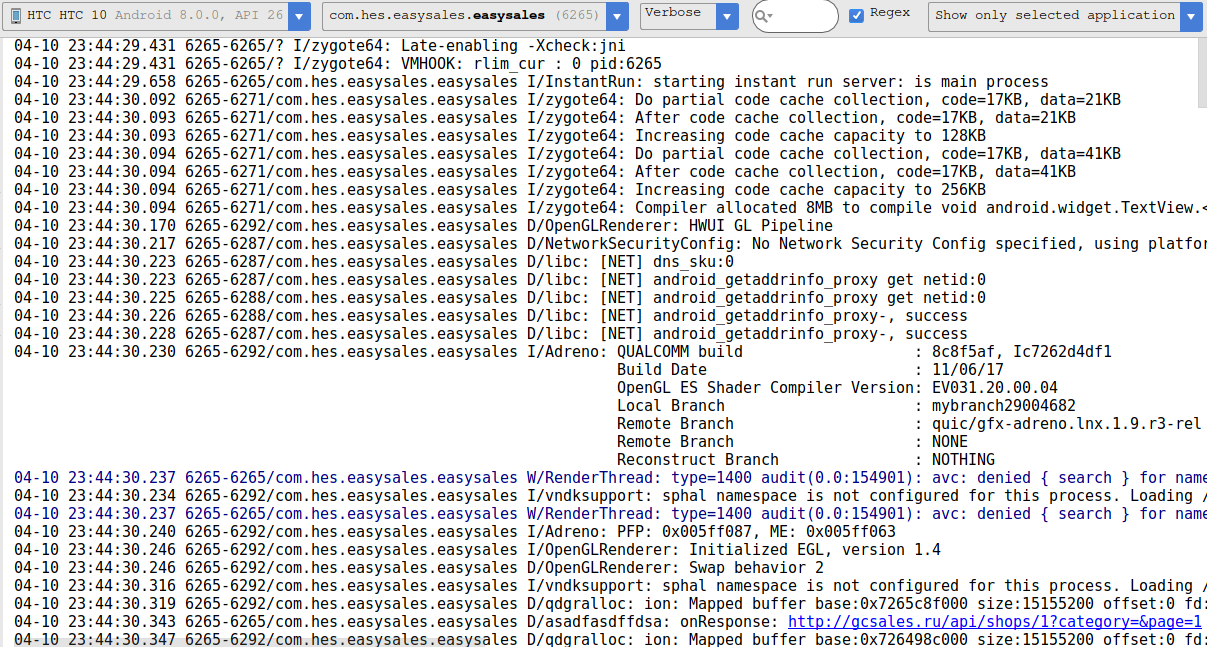
\includegraphics[width=0.9\textwidth]{./screenshots/3/lauch_log.png}
    \caption{\small{log. Запуск приложения}}
    \label{launch}
\end{figure}


Время загрузки одной страницы акций не должно превышать двух секунд (Рис.~\ref{loading})

\begin{figure}[h!]
    \centering
    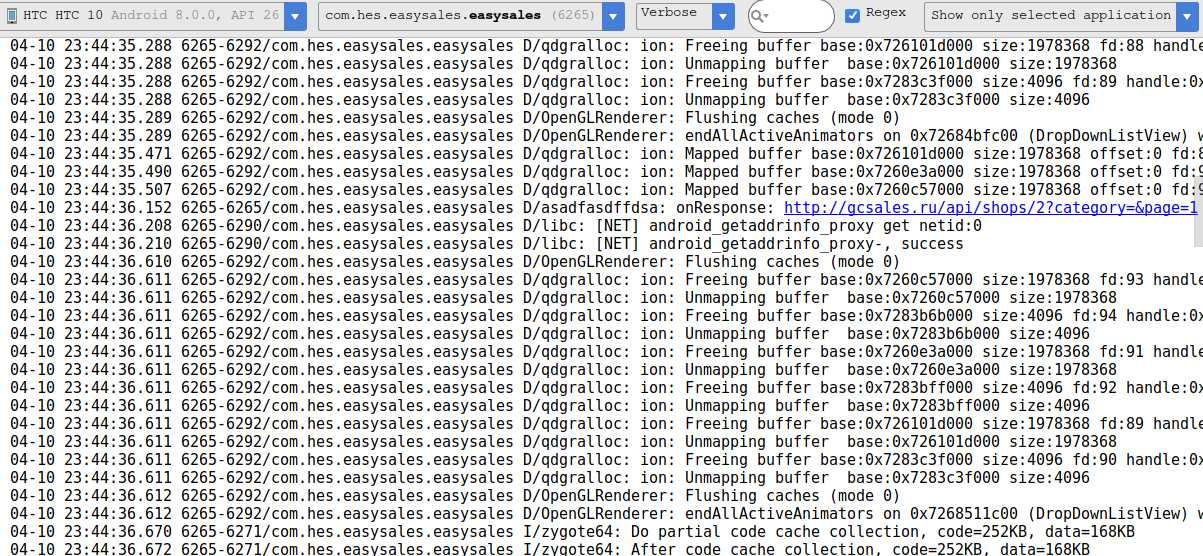
\includegraphics[width=0.9\textwidth]{./screenshots/3/load_log.png}
    \caption{\small{log. Загрузка акций}}
    \label{loading}
\end{figure}
Все временные требования должны быть соблюдены.
\subsubsection{Crawler}
Временные требования к работе crawler'a не предъявлялись.


\newpage
\section{Приложение 1. Терминология}
\subsection{Терминология}
\begin{description}
  \item[REST (от англ. Representational State Transfer)] -- способ сетевого
    взаимодействия.  REST API определяет набор функций, к которым разработчики
    могут совершать запросы и получать ответы. Взаимодействие происходит по
    протоколу HTTP.  Преимуществом такого подхода является широкое
    распространение протокола HTTP, поэтому REST API можно использовать
    практически из любого языка программирования.
\end{description}



\newpage
\section{Приложение 2. Список используемой литературы}
\subsection{Список используемой литературы}
\begin{my_enumerate}
    \item
    ГОСТ 19.102-77 Стадии разработки. //Единая система программной документации. -М.: ИПК Издательство стандартов, 2001.
    
    \item
    ГОСТ 19.201-78 Техническое задание. Требования к содержанию и оформлению // Единая система программной документации. -М.:ИПК Издательство стандартов, 2001.
    
    \item  ГОСТ 19.404-79 Пояснительная записка. Требования к содержанию и оформлению. //Единая система программной документации. – М.: ИПК Издательство стандартов, 2001
    
    \item
    ГОСТ 19.101-77 Виды программ и программных документов
    //Единая система программной документации. -М.: ИПК Издательство стандартов, 2.: 001.
    
    \item
    ГОСТ 19.103-77 Обозначения программ и программных документов. //Единая система программной документации. -М.: ИПК Издательство стандартов, 2001.
    
    \item
    ГОСТ 19.104-78 Основные надписи //Единая система программной документации. -М.: ИПК Издательство стандартов, 2001.
    
    \item 
    ГОСТ 19.106-78 Требования к программным документам, выполненным печатным способом. //Единая
    система программной документации. – М.: ИПК Издательство стандартов, 2001
    
    \item 
    ГОСТ 19.603-78 Общие правила внесения изменений. //Единая система программной документации. –
    М.: ИПК Издательство стандартов, 2001
    
    \item
    Oculus Documentation [Электронный ресурс]: Режим доступа: https:// developer3.oculus. com/documentation/
    
    \item
    Oculus Developers Blog [Электронный ресурс]: chrispruett – Squeezing Performance out of your Unity Gear VR Game, 2015 - Режим доступа: https://developer3.oculus.com/blog /squeezing-performance-out-of-your-unity-gear-vr-game/
    
    \item 
    Uninty Scripting Reference [Электронный ресурс]: Режим доступа: https: //docs.unity3d. com/ScriptReference/
    
\end{my_enumerate}




% Index
\newpage
\eskdListOfChanges

% \phantomsection
% \addcontentsline{toc}{section}{Алфавитный указатель}
% \printindex

\end{document}
